\documentclass[linenumbers]{aastex631}

\usepackage{amsmath}

\shorttitle{Dark energy is based on a math error from 1930}
\shortauthors{Evans}

\begin{document}

\title{Dark energy is based on a math error from 1930}

\correspondingauthor{Logan P. Evans}
\email{loganpevans@gmail.com}

\author[0000-0001-6450-3262]{Logan P. Evans}

\begin{abstract}
We show that the apparent magnitude of distant objects has been calculated
incorrectly since 1930. We describe how this redshift correction flaw in the
formula for K-corrections has propagated for over nine decades. We also
re-derive the K-corrections equation. This derivation reveals that the
correction for zero-points in different filters also has a flaw. We explore the
consequences of properly correcting apparant magnitudes for redshift and
conclude that this resolves two of the preeminent mysteries in cosmology: dark
energy is not supported by observations of Type Ia supernovae, and the Hubble
tension is due to a calculation error.
\end{abstract}

%% https://astrothesaurus.org
\keywords{Type Ia supernovae(1728) --- Apparent magnitude(59)}

\section{Introduction}

The measurement of Type Ia supernovae is one of the primary sources of data for
cosmological models. The measurements involve estimating the peak magnitude in
the B filter \citet{riess1998} for the rest frame, meaning we want to know how
bright the SnIa would be if its light did not undergo redshift. Redshift causes
the light that would be measured by the B filter in a rest frame to be shifted
to another filter. In order to observe a SnIa in an arbitrary filter and report
the magnitude in the B filter we use a technique called K-corrections.

The first formal derivation of K-corrections was performed by
\citet{tolman1930} and it failed to account for bandwidth stretching, one of
the dimming effects of redshift. This error was noted by \citet{desitter1934},
but in \citet{hubble1935} the discrepancy was noted and ignored.
\citet{oke1968} rederived K-corrections, but they failed to account for time
dilation, one of the other dimming effects of redshift. In \citet{kim1996},
K-corrections were extended to handle additional cross-filter comparisons and
address zero-point corrections, but they started their derivation by
referencing the incorrect equation from \citet{oke1968}. The derivation in
\citet{kim1996} forms the basis for modern implementations of K-corrections.
This history is explored in more depth in Section \ref{sec:history}.

The effect of using an incorrect magnitude for SnIa is that we think objects
are farther away than they really are, and the effect compounds for greater
distances. Up until \citet{riess1998}, we didn't have distant enough
observations for this error to matter much for cosmology models, but in the
late 1990s, it was clear that our measurements for distance and redshift were
not linear. This observation led to a model that utilized a cosmological
constant and dark energy in order to explain the non-linear distance-redshift
graph. We will show in Section \ref{sec:tension} that correcting the flaw
with K-corrections leads to a linear graph that does not need to rely on a
cosmological constant.

\citet{planck2020} used an alternative technique to compute the Hubble constant
that is based on measurements of the cosmic microwave background. CMB based
computations of $H0$ has made it evident that something was missing with our
understanding of cosmology because this measurement is incompatible with the
Hubble constant when measured from SnIa. As we will discuss in Section
\ref{sec:tension}, fixing the error with K-corrections produces a measurement
of the Hubble constant that is compatible with models based on the cosmic
microwave background.

\section{A brief history of K-corrections}
\label{sec:history}

Observations of Type Ia supernova are essential to calibrate models that
measure redshift and estimate distance. This relationship, often called the
Hubble-Lema\^{i}tre law, describes how quickly the universe is expanding.
However, \citet{riess1998} and \citet{perlmutter1999} presented evidence that
there isn't a linear relationship between redshift and distance, but instead,
distant objects are farther away than their redshift would predict (see Figure
\ref{fig:mu_distance_vs_redshift}). This phenomenon implies that the
acceleration of the universe is faster today than it was for old observations.
Previously the cause of this phenomenon was unknown and was referred to as
dark energy.

\begin{figure}
  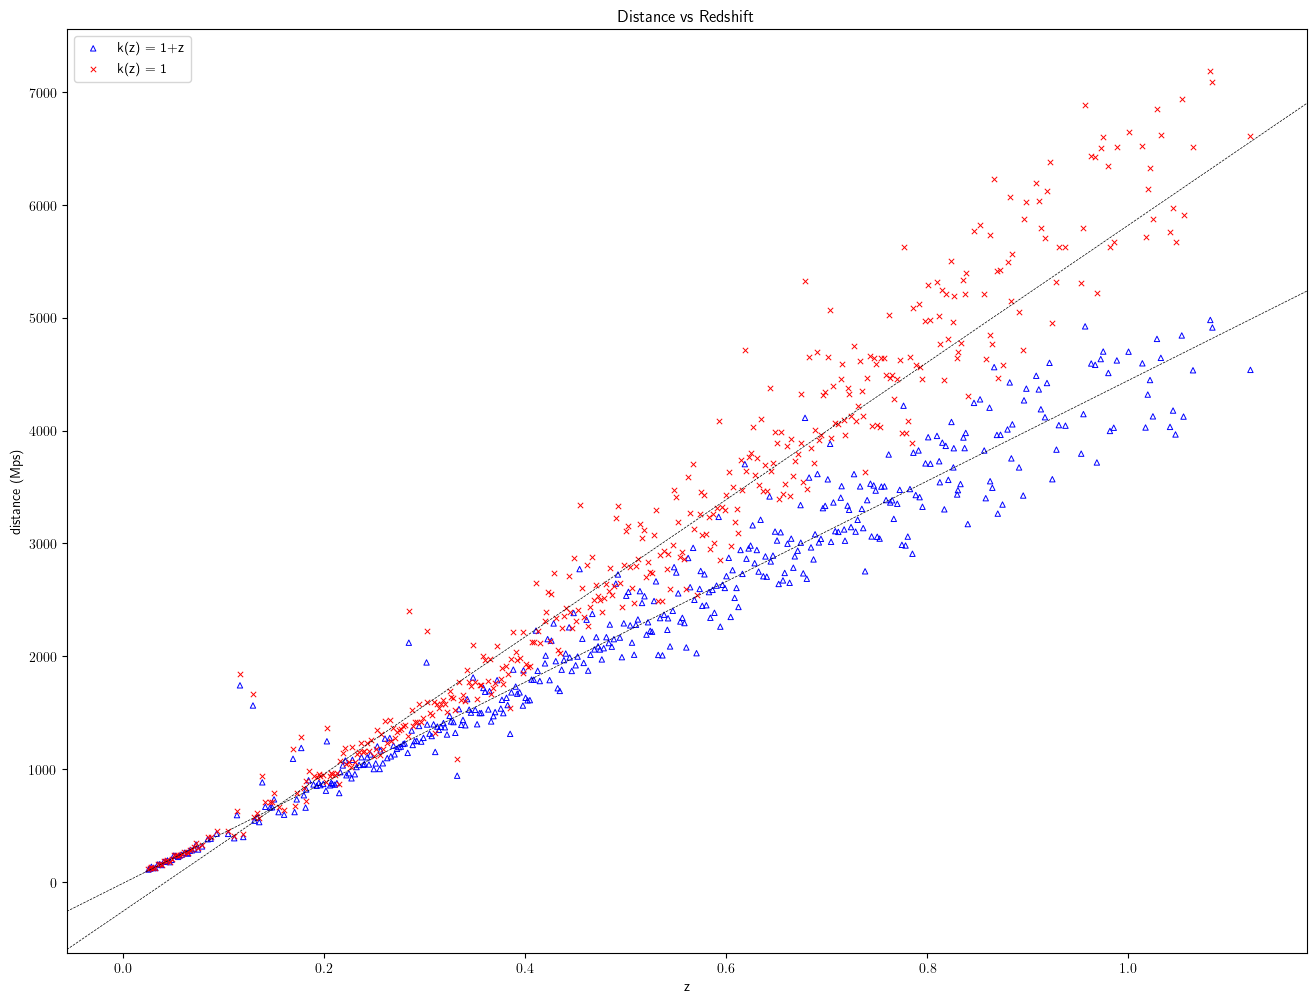
\includegraphics[width=\linewidth]{mu_distance_vs_redshift.png}
  \caption{The relationship between distance and redshift for two treatments of
  magnitude data. The displayed points are roughly a third of the values in the
  full SnIa dataset published in \citet{abbott2024}, selected evenly to aid
  visibility. The $k(z) = 1$ treatment, which represents the uncorrected
  values, is clearly non-linear while the $k(z) = 1 + z$ treatment which fixes
  the K-correction redshift error, appears to be linear.}
  \label{fig:mu_distance_vs_redshift}
\end{figure}

Type Ia supernovae are used to explore the relationship between distances and
redshifts because these events always happen in similar ways, so the absolute
brightness is roughly always the same. An analogy is to imagine someone walking
in the dark and lighting matches. As long as we know how brightly a match burns
at a known distance, we can estimate the distance to any match by measuring the
apparent brightness before applying some geometry.

However, redshifting light dims an observation in three ways:

\begin{itemize}
  \item The energy of a wave is inversely proportional to its wavelength, so a
  redshift of $z$ means the amount of energy per photon is reduced by a factor
  of $\frac{1}{1+z}$.

  \item The bandwidth is stretched out. If a rest frame would observe photons
  between teh wavelengths of 400nm and 401nm, then with a redshift of $z = 1$,
  redshifting these photons will spread them across the wavelengths from 800nm
  to 802nm.

  \item Cosmological time dilation reduces the rate at which photons arive.
\end{itemize}

To complicate matters, we use the B-band magnitude to calculate luminosity
distance. We want to know how bright a supernova appears for wavelengths around
445nm as if no redshift had occured. However, we typically need to observe the
supernova with a filter that is sensitive to longer wavelengths, such as the
i-band filter which is sensitive to wavelengths from 700nm-850nm
\citep{flaugher2015}. The K-corrections formula allows us to take a magnitude
measured in an observation filter $y$ and compute the magnitude in the target
filter $y$.

The first mathematical treatments of K-corrections was performed by
\citet{tolman1930}. However, when Tolman made his derivation, he did not
consider the effects of a spectra that is stretched out due to redshift. See
the top two panels of Figure \ref{fig:k-example} for an example of this effect.

A few years later, \citet{desitter1934}, discussed all three issues that reduce
the observed magnitude of a distant observation. The correction for each of
these issues is identical: take a measurement for luminosity and multiply it by
the factor $1 + z$.

A year later, \citet{hubble1935} published a similar set of calculations for
K-corrections, but these equations used $(1 + z)^2$ instead of the $(1 + z)^3$
correction term used by de Sitter. They started their derivation by copying the
incorrect equation from 1930. After their derivation, they noted,

\begin{quote}
It should be specially noted that this expression differs from the correction
to $m$ proposed by de Sitter, which contains the term $(1 + z)^3$ instead of
$(1 + z)^2$. Expression (28), however, would seem to give the proper correction
to use in connection with our equation (21), since it has been derived in such
a way as to make appropriate allowance, first, for the double effect of nebular
recession in reducing both the individual energy and the rate of arrival of
photons, and then for the further circumstance that a change in spectral
distribution of the energy that does arrive will lead to changes in its
photographic effectiveness.
\end{quote}

The Hubble K-corrections with the incorrect correction term have been used ever
since.

By \citet{oke1968}, the two factors of $(1 + z)$ were attributed to the change
in energy and to the spectral bandwidth elongation, which leaves time dilation
as the factor that was omitted. A graph that demonstrates why it's essential to
correct for both the spectra bandwidth warping and time dilation is presented
in Figure \ref{fig:k-example}.

\begin{figure}
  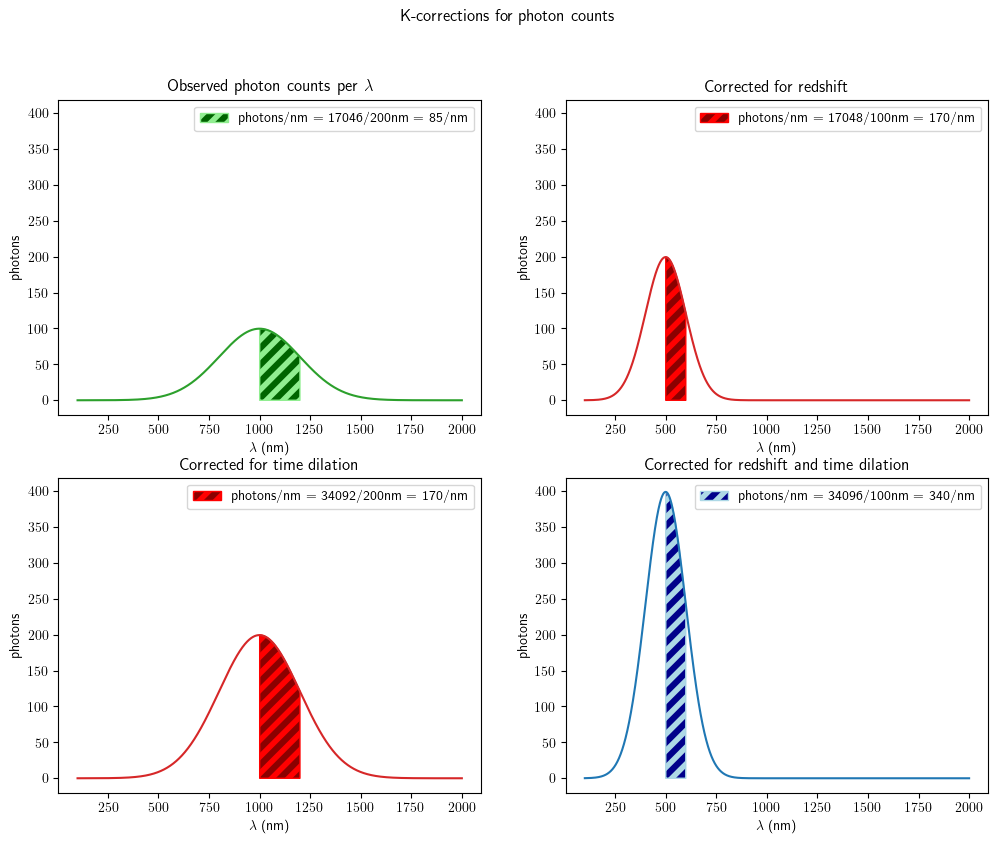
\includegraphics[width=.75\linewidth]{K-corrections_for_photon_counts.png}
  \caption{An example of how K-corrections take an observed magnitude and
  produce a rest frame magnitude. In this example, $z=1$. The observation
  filter measures magnitude, which is equivalent to measuring the number of
  photons per nanometer. In the bottom left panel, a correction of $1+z$ is
  applied which doubles the photons per nanometer. The top right panel shows
  the effect of correcting for the bandwidth spectrum warping effect --
  correcting all wavelengths for the rest frame means that the measured
  wavelengths have blueshifted, ideally into the cross band B filter. Applying
  both effects, shown in the bottom right panel, requires applying two
  correction factors of $1+z$. This example omits the correction for a similar
  effect related to lower energy due to the Planck relation because CCD cameras
  obviate the need to correct for this effect.
  }
  \label{fig:k-example}
\end{figure}

The modern treatment of K-corrections is based on the work of \citet{kim1996}.
This work extended the calculations of K-corrections to extend to filters
beyond B and V. It also introduced a term that deals with the zero-point for
the actual filters. In the modern day, filters measure the photon flux as
opposed to the energy flux. Historically, bolometric devices would measure the
energy flux, but modern CCD cameras effectively measure the photon flux.

Quoting \citet{kim1996}:

\begin{quote}
  Therefore, the correct K correction calculation to be used with measured
  photometric magnitudes is the integral photon counts:

  \begin{equation}
  \label{eq:kim}
    K_{xy} =
      -2.5\text{log} \left(
        \frac{\int \lambda \mathcal{Z}(\lambda)S_x(\lambda)d\lambda}
             {\int \lambda \mathcal{Z}(\lambda)S_y(\lambda)d\lambda}\right)
      + 2.5\text{log}(1+z)
      + 2.5\text{log}\left(
        \frac{\int \lambda F(\lambda)S_x(\lambda)d\lambda}
             {\int \lambda F(\lambda/(1+z))S_y(\lambda))d\lambda}\right).
  \end{equation}
\end{quote}

This equation has three errors, which we will explore in Section
\ref{sec:consequences}.

\section{Derivation of K-corrections}
\label{sec:derivation}

With modern CCD cameras, a telescope observation consists of a single value
$\mathcal{F}_x$ erg/s, which represents the energy collected in filter $x$ per
second. A summary of how this works is provided by \citet{lesser2015}. The
measured energy is produced by electrons not photons, so the measured number is
proportional to the number of photons. However, we need to calculate the
expected number of photons collected by using a spectral energy density
function $F$. The value $F(\lambda)$ gives the amount of energy collected by a
bolometric device for the wavelength $\lambda$.

To convert the spectral energy density $F$ to the photon density $F'$, we need
to use the Plank relation $E = \frac{hc}{\lambda}$ where $E$ is the energy, $h$
is Planck's constant, and $c$ is the speed of light. This gives us

\begin{equation}
\begin{aligned}
   F(\lambda) &= F'(\lambda) \times \frac{hc}{\lambda} \\
  F'(\lambda) &= \frac{\lambda F(\lambda)}{hc}.
\end{aligned}
\end{equation}

It's important to note that for the blueshifted wavelength $\lambda / (1+z)$,
this equation produces

\begin{equation}
 F'\left(\frac{\lambda}{1+z}\right) = \frac{\lambda}{(1+z)hc} F\left(\frac{\lambda}{1+z}\right).
\end{equation}

However, this equation is misleading and error prone. We will want to use it to
help calculate the amount of flux in an observation filter at the redshifted
wavelength $\lambda \times (1 + z)$. In other words, we want to produce the
photon density function $R'$ that is the redshifted version of $F'$.
Redshifting the photon density does two things:

\begin{itemize}
  \item The stretching of space increases the distance between photons while
  they are traveling. This phenomenon appears to an observer like time
  dilation, although cosmological time dilation is due to a different mechanism
  than relativistic time dilation. This effect reduces the photon arrival rate
  by a factor of $1/(1+z)$.

  In order to account for cosmological time dilation, we will need to multiply
  $F'$ by $1/(1+z)$.

  \item All wavelengths are changed by a factor of $1 + z$. When we integrate
  $R'$ from wavelength $\lambda_a$ to wavelength $\lambda_b$, the values
  correspond to the wavelengths $\lambda_a / (1+z)$ to $\lambda_b / (1+z)$ in
  $F'$. We will integrate over a width of $\lambda_b - \lambda_a$, but
  $F'(\lambda / (1+z))$ will refer to values in a width of
  $(\lambda_b - \lambda_a) / (1+z)$.

  In order to account for this bandwidth spectral warping effect, we will need
  to multiply $F'$ by a second factor of $1/(1+z)$.
\end{itemize}

Combining these two phenomena together, we can calculate the redshifted
spectral energy density $R$ using

\begin{equation}
\begin{aligned}
\label{eq:redshifted_density}
  R'(\lambda) &= F'\left(\frac{\lambda}{1+z}\right) \times \frac{1}{(1 + z)^2} \\
  R(\lambda) &= \frac{\lambda}{(1+z)hc} \times F\left(\frac{\lambda}{1+z}\right) \times \frac{1}{(1 + z)^2} .
\end{aligned}
\end{equation}

We deliberately do not combine all of the factors of $1+z$ together because
this form is more natural to implement in code.

In order to calculate the amount of flux $\mathcal{F}_x$ measured in filter
$x$, we need to compute the photon density $F'(\lambda)$ and multiply it by
sensitivity $S_x(\lambda)$, which represents the proportion of photons filter $x$
will measure at wavelength $\lambda$. We then need to sum over all wavelengths,
which is expressed with the equation

\begin{equation}
\begin{aligned}
\label{eq:flux_definition}
  \mathcal{F}_x &= \int F'(\lambda) S_x(\lambda) d\lambda \\
                &= \int \lambda F(\lambda) S_x(\lambda) d\lambda.
\end{aligned}
\end{equation}

The limits of integration are technically from 0 to $\infty$, but these are
usually not written because the sensitivity $S(\lambda)$ is 0 for wavelengths
outside of a filter's bandpass.

We will also use the energy flux $\mathcal{F}$ to magnitude $m$ formula:

\begin{equation}
\begin{aligned}
\label{eq:flux2mag}
                             m_x &= -2.5 \text{log}(\mathcal{F}_x) + P_x \\
  -2.5 \text{log}(\mathcal{F}_x) &= m_x - P_x .
\end{aligned}
\end{equation}

$P_x$ represents the zero-point for the filter $x$ on some particular
telescope. In order to use consistent magnitude values across telescopes that
have different light gathering abilities, we take the measured magnitude and
multiply it by the ratio of the standard flux rate to the flux rate for this
particular telescope and filter. For convenience, we use $P_x = -2.5
\text{log}(P'_x)$ so that we can work with flux instead of with magnitude.

Now that we have the identities in Equations \ref{eq:flux_definition} and
\ref{eq:flux2mag} we will change directions and look at the definition of
K-corrections $K_{xy}$. This value allows us to make an observation in filter
$y$ and report what the magnitude would have been in filter $x$ if no redshift
occured:

\begin{equation}
\begin{aligned}
\label{eq:definition}
  m_y &= M_x + \mu + K_{xy} \\
      &= M_x + m_x - M_x + K_{xy} \\
      &= m_x + K_{xy} \\
  m_x &= m_y - K_{xy} .
\end{aligned}
\end{equation}

The second line of Equation \ref{eq:definition} expands the distance modulus
$\mu$ using $\mu = m - M$ where $m$ is the observed magnitude and $M$ is the
absolute magnitude.

Since the K-correction is a magnitude value and we wish to work on flux values,
it is convenient to define the following substitution:

\begin{equation}
\label{eq:k_substitution}
  K_{xy} = 2.5\text{log}(K'_{xy}) .
\end{equation}

Note that this substitution omits the minus ($-$) sign that we used on a
similar substitution for $P_x$.

Starting with Equation \ref{eq:flux2mag} and then
recombining the flux term $\mathcal{F}_y$ with $m_y$ from Equation
\ref{eq:definition}, we have

\begin{equation}
\begin{aligned}
\label{eq:as_flux}
  -2.5 \text{log}(\mathcal{F}_x)
      &= m_x - P_x \\
      &= m_y - K_{xy} - P_x \\
      &= -2.5 \text{log}(\mathcal{F}_y) + P_y - K_{xy} - P_x \\
      &= -2.5 \text{log}(\mathcal{F}_y)
         - 2.5 \text{log}(P'_y)
         - 2.5 \text{log}(K'_{xy})
         + 2.5 \text{log}(P_x) \\
      &= -2.5 \left(
         \text{log}(\mathcal{F}_y)
         + \text{log}(K'_{xy})
         + \text{log}(P'_y)
         - \text{log}(P'_x)
        \right) \\
      &= -2.5 \text{log}\left(
        \mathcal{F}_y
        \times K'_{xy}
        \times \frac{P'_y}{P'_x}\right) \\
  \mathcal{F}_x &= \mathcal{F}_y \times K'_{xy} \times \frac{P'_y}{P'_x}.
\end{aligned}
\end{equation}

It's useful to inspect this equation to consider whether the term
$\frac{P'_y}{P'_x}$ is correct, or if it might be flipped to the inverse of
what it should be. However, if we rewrite Equation \ref{eq:as_flux} as

\begin{equation}
  \mathcal{F}_x \times P'_x = \mathcal{F}_y \times P'_y \times K'_{xy}
\end{equation}

\noindent then the meaning is a bit more clear. The left hand side
$\mathcal{F}_x \times P'_x$ is the rate of photon collection for an idealized
telescope in filter $x$ while $\mathcal{F}_y \times P'_y$ is the rate of photon
collection for an idealized telescope in filter $y$. We are able to observe the
value $\mathcal{F}_y \times P'_y$ and want to use the fudge factor $K'_{xy}$ to
produce the value $\mathcal{F}_x \times P'_x$.

We can isolate $K'_{xy}$ and then use Equation \ref{eq:flux_definition} to expand

\begin{equation}
\begin{aligned}
  \mathcal{F}_x &= \mathcal{F}_y \times K'_{xy} \times \frac{P'_y}{P'_x} \\
        K'_{xy} &= \frac{P'_x}{P'_y} \times \frac{\mathcal{F}_x}{\mathcal{F}_y} .
\end{aligned}
\end{equation}

Now we use Equations \ref{eq:redshifted_density} and \ref{eq:flux_definition}
to calculate the fluxes $\mathcal{F}_x$ and $\mathcal{F}_y$ in terms of the
spectral energy density function $F$. Note that $\mathcal{F}_x$ uses the rest
frame spectral energy density $F$ while $\mathcal{F}_y$ uses the redshifted
spectral energy density $R(\lambda)$:

\begin{equation}
\begin{aligned}
  K'_{xy} &= \frac{P'_x}{P'_y} \times \frac{\mathcal{F}_x}{\mathcal{F}_y} \\
         &= \frac{P'_x}{P'_y} \times
              \frac{\int F'(\lambda) S_x(\lambda) d\lambda}
                   {\int R'(\lambda) S_y(\lambda) d\lambda} \\
         &= \frac{P'_x}{P'_y} \times
              \frac{\int F'(\lambda) S_x(\lambda) d\lambda}
                   {\int F'(\frac{\lambda}{1+z}) \times \frac{1}{(1 + z)^2} S_y(\lambda) d\lambda} \\
         &= \frac{P'_x}{P'_y} \times (1+z)^2 \times
              \frac{\int \frac{\lambda}{hc} F(\lambda) S_x(\lambda) d\lambda}
                   {\int \frac{\lambda}{(1+z)hc} F\left(\frac{\lambda}{1+z}\right) S_y(\lambda) d\lambda} \\
         &= \frac{P'_x}{P'_y} \times (1 + z)^2 \times
              \frac{\int \lambda F(\lambda) S_x(\lambda) d\lambda}
                   {\int \frac{\lambda}{1+z} F\left(\frac{\lambda}{1+z}\right) S_y(\lambda) d\lambda} .
\end{aligned}
\end{equation}

Finally, we can use Equation \ref{eq:k_substitution} to convert the flux $K'_{xy}$ back
into the magnitude $K_{xy}$:

\begin{equation}
\begin{aligned}
\label{eq:K2k}
  K_{xy} &= 2.5\text{log}(K'_{xy}) \\
         &= 2.5\text{log}\left(
            \frac{P'_x}{P'_y} \times (1 + z)^2 \times
            \frac{\int \lambda F(\lambda) S_x(\lambda) d\lambda}
                 {\int \frac{\lambda}{1+z} F\left(\frac{\lambda}{1+z}\right) S_y(\lambda) d\lambda}\right) \\
         &= 2.5 \left(
            \text{log} \left( \frac{P'_x}{P'_y} \right)
            + \text{log}( {(1 + z)^2})
            + \text{log}\left( \frac{\int \lambda F(\lambda) S_x(\lambda) d\lambda}
                   {\int \frac{\lambda}{1+z} F\left(\frac{\lambda}{1+z}\right) S_y(\lambda) d\lambda}
            \right) \right) \\
         &= 2.5 \text{log} \left( \frac{P'_x}{P'_y} \right)
            + 5 \text{log} (1 + z)
            + 2.5 \text{log} \left(
              \frac{\int \lambda F(\lambda) S_x(\lambda) d\lambda}
                   {\int \frac{\lambda}{1+z} F\left(\frac{\lambda}{1+z}\right) S_y(\lambda) d\lambda} \right) \\
         &= 5 \text{log} (1 + z)
            + 2.5 \text{log} \left(
              \frac{\int \lambda F(\lambda) S_x(\lambda) d\lambda}
                   {\int \frac{\lambda}{1+z} F\left(\frac{\lambda}{1+z}\right) S_y(\lambda) d\lambda} \right)
            - P_x + P_y .
\end{aligned}
\end{equation}

\section{Consequences}
\label{sec:consequences}

In order to fully compare our derivation against Equation \ref{eq:kim}, we need
to use the identity

\begin{equation}
  P = -2.5 \text{log} \left( \int \frac{\lambda}{hc} \mathcal{Z}(\lambda) S(\lambda) d\lambda \right)
\end{equation}

\noindent where, according to \citet{kim1996}, "$\mathcal{Z}(\lambda)$ is an
idealized spectral energy distribution at $z = 0$ for which
$U = B = V = R = I = 0$ in the photometric system being used." Combining this
with Equation \ref{eq:K2k}, we have

\begin{equation}
\begin{aligned}
  K_{xy} &= 5 \text{log} (1 + z)
            + 2.5 \text{log} \left(
              \frac{\int \lambda F(\lambda) S_x(\lambda) d\lambda}
                   {\int \frac{\lambda}{1+z} F\left(\frac{\lambda}{1+z}\right) S_y(\lambda) d\lambda} \right)
            - P_x + P_y \\
         &= 5 \text{log} (1 + z)
            + 2.5 \text{log} \left(
              \frac{\int \lambda F(\lambda) S_x(\lambda) d\lambda}
                   {\int \frac{\lambda}{1+z} F\left(\frac{\lambda}{1+z}\right) S_y(\lambda) d\lambda} \right)
            + 2.5 \text{log} \left( \int \frac{\lambda}{hc} \mathcal{Z}(\lambda) S_x(\lambda) d\lambda \right)
            - 2.5 \text{log} \left( \int \frac{\lambda}{hc} \mathcal{Z}(\lambda) S_y(\lambda) d\lambda \right) \\
         &= 2.5 \text{log} \left(
              \frac{\int \lambda \mathcal{Z}(\lambda) S_x(\lambda) d\lambda}
                   {\int \lambda \mathcal{Z}(\lambda) S_y(\lambda) d\lambda}
             \right)
            + 5 \text{log} (1 + z)
            + 2.5 \text{log} \left(
              \frac{\int \lambda F(\lambda) S_x(\lambda) d\lambda}
                   {\int \frac{\lambda}{1+z} F\left(\frac{\lambda}{1+z}\right) S_y(\lambda) d\lambda} \right) .
\end{aligned}
\end{equation}

Three differences with Equation \ref{eq:kim} stand out:

\begin{itemize}
  \item The sign is different for the first term. This will have a subtle but
  frustrating effect for real measurements. Typically the zero-point values are
  similar, so this term is close to 0. However, the term isn't always zero. As
  we observe more distant supernovae, it is useful to switch our observational
  filter to a filter that is sensitive to longer wavelengths. Each observation
  filter will have its own small bias.

  This effect by itself can alter estimates of $H_0$ by several km/s / Mpc.
  While we present an estimate of the Hubble constant in Figure
  \ref{fig:H0bootstrap}, we aren't terribly confident in the numbers because we
  were unable to correct for the zero-point correction errors or verify that
  these errors don't exist.

  \item The second term is multiplied by a $2.5$ in \citet{kim1996} but is
  multiplied by a $5$ here. This is the manifestation of the error in
  \citet{tolman1930}.

  \item In our derivation, the third term is has an extra $1 + z$ expression.
  Based on an inspection of the SN(oo)py software package presented by
  \citet{snpy}, this error is ignored and software package authors implement it
  as the expression is intended, not precisely as the expression is written.
\end{itemize}

\section{Dark energy and the Hubble tension}
\label{sec:tension}

As shown in Figure \ref{fig:mu_distance_vs_redshift}, when reported magnitudes
are corrected by adding the magnitude $-2.5\text{log}(1+z)$, there is a linear
relationship between redshift and luminosity distance. This is in accordance
with the Hubble-Lema\^{i}tre law. As opposed to the uncorrected values, there
is no visual acceleration.

Since the corrected values are approximately linear, we can use them to
estimate the Hubble constant $H0$. This is demonstrated in Figure
\ref{fig:expansion}. Furthermore, we performed a bootstrap calculation to
estimate the distribution of $H0$ estimates in Figure \ref{fig:H0bootstrap}.

The value estimated here, $H0 \sim 65.94 \pm 1.29$ is highly suspicious because
of the flipped zero-point corrections, but it is consistent with estimates of
$H0$ that are based on the CMB. \citet{planck2020} published the CMB value of
$H0 \sim 67.27 \pm 0.6$, and the one sigma error bars overlap. It is
interesting to note that restricting the DES observations to only those with $z
< 0.1$, which presumably is a small enough redshift that all observations will
have been made with the same filter, gives the estimate
$H0 \sim 67.8 \pm 1.86$.

\begin{figure}
  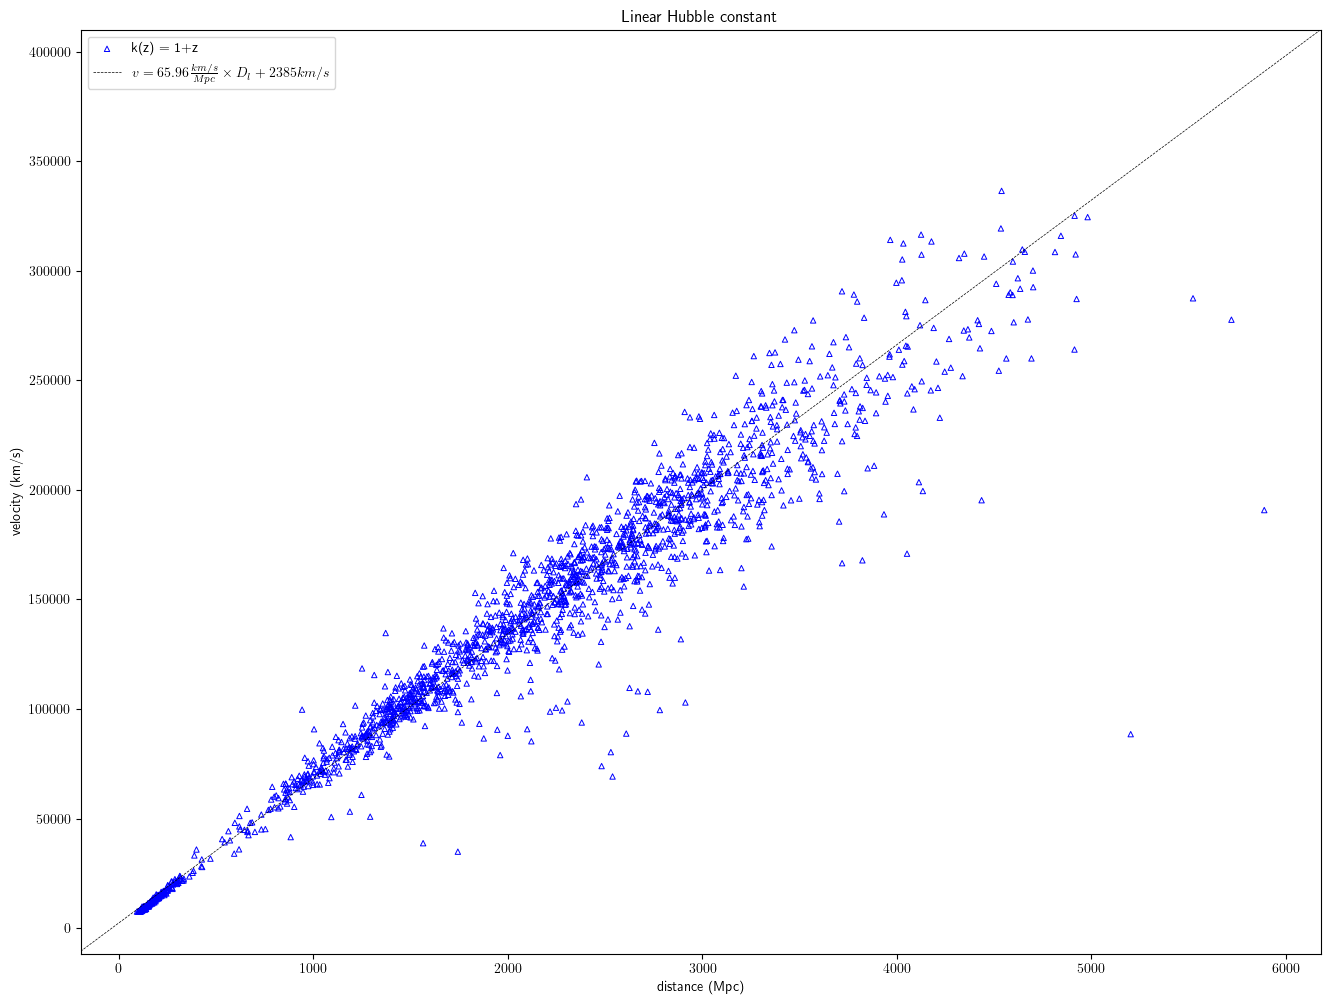
\includegraphics[width=\linewidth]{velocity_vs_distance.png}
  \caption{The relationship between expansion velocity and distance. The slope of this graph demonstrates the Hubble constant.
  }
\label{fig:expansion}
\end{figure}

\begin{figure}
  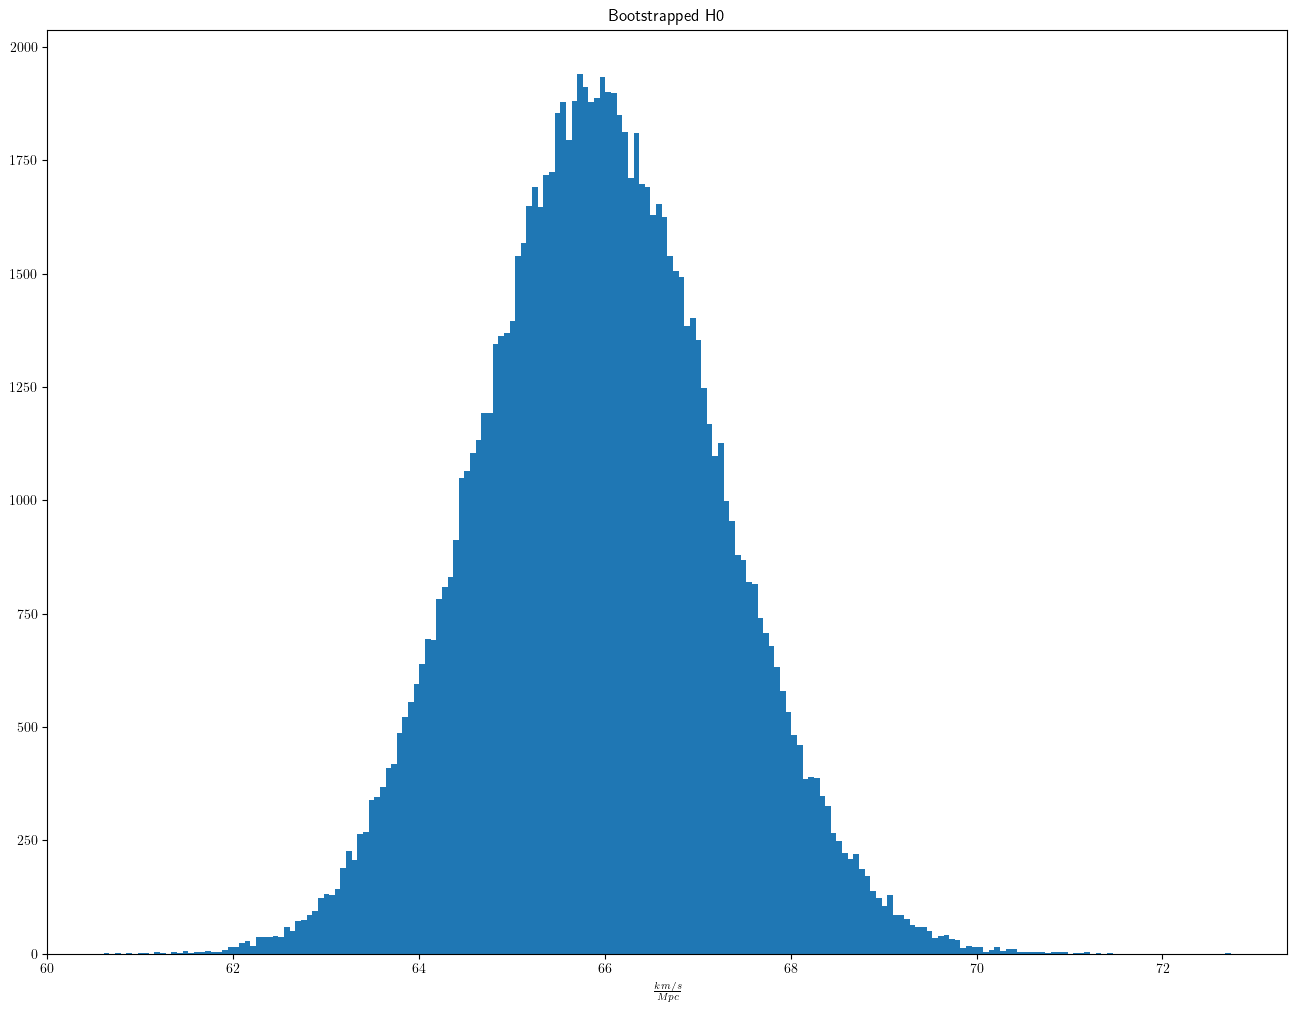
\includegraphics[width=\linewidth]{bootstrapped_H0.png}
  \caption{A histogram of 100000 bootstrap trials measuring the Hubble constant
  $H0$. Each trial samples an absolute Type Ia magnitude $M \sim Norm(-19.2334,
  0.0404)$ based on data published by \citet{camarena2020}. It then samples,
  with replacement, a population of supernovae from the dataset published by
  \citet{abbott2024}. Finally, it uses the non-parametric linear regression
  technique described by \citet{siegel1982}. The result of the bootstrap is $H0
  \sim Norm(65.94, 1.29^2)$.
  }
\label{fig:H0bootstrap}
\end{figure}

\section{Conclusions}

A lot of data is going to have to be reanalyzed.

\bibliography{references}{}
\bibliographystyle{aasjournal}

\end{document}
